\documentclass[a4paper,12pt]{article}
\usepackage{a4wide}
\usepackage{acronym}
\usepackage{graphicx}
\usepackage[title,titletoc,toc]{appendix}


\begin{document}

\begin{titlepage}
\begin{center}
\vspace*{3cm}
{\LARGE\bf Travelling Salesman Problem}\\
\vspace{1.5cm}
{\large\bf for}\\
\vspace{1.5cm}
{\LARGE\bf Evolutionary Computation}\\
\vspace{5cm}
Prepared by William Reid, Matthew Hart, Samantha Peachey \& Alec Bellati\\
\vspace{1cm}
School of Computer Science,\\
The University of Adelaide\\
\vspace{1cm}
\today
\end{center}
\end{titlepage}
%\thispagestyleempty


\section{Introduction}

After much discussion amongst the project team, three algorithms were formulated. But it was evident that some of them relied on some type of percentage values. Given we had little experience in what these percentages would be or could mean, we decided on running the operators and mutators multiple times on a simple data set to ascertain how they performed. The steps taken to acquire this data are as follows:
\begin{enumerate}
\item Each run was performed 10 times, with a population of 50 and for 10,000 generations.
\item For each run, the mutators/operator would begin at 0\% (chance of being selected). If the mutators/operator was not selected, no operation would occur for that cycle.
\item This chance of being selected would increase by 5\% after set of 10 runs
\item Once the probability of being selected had reached 100\%, the tests began on the next operator/mutator.
\item Each mutators/operator was tested
\item Steps 1-5 were repeated for each selection method.
\end{enumerate}

This provided us with 8 graphs, with the most significant – Edge Recombination – shown below. The remaining graphs have been ommited from this report but can be obtained from the team if required.

\begin{figure}[h]
\centering
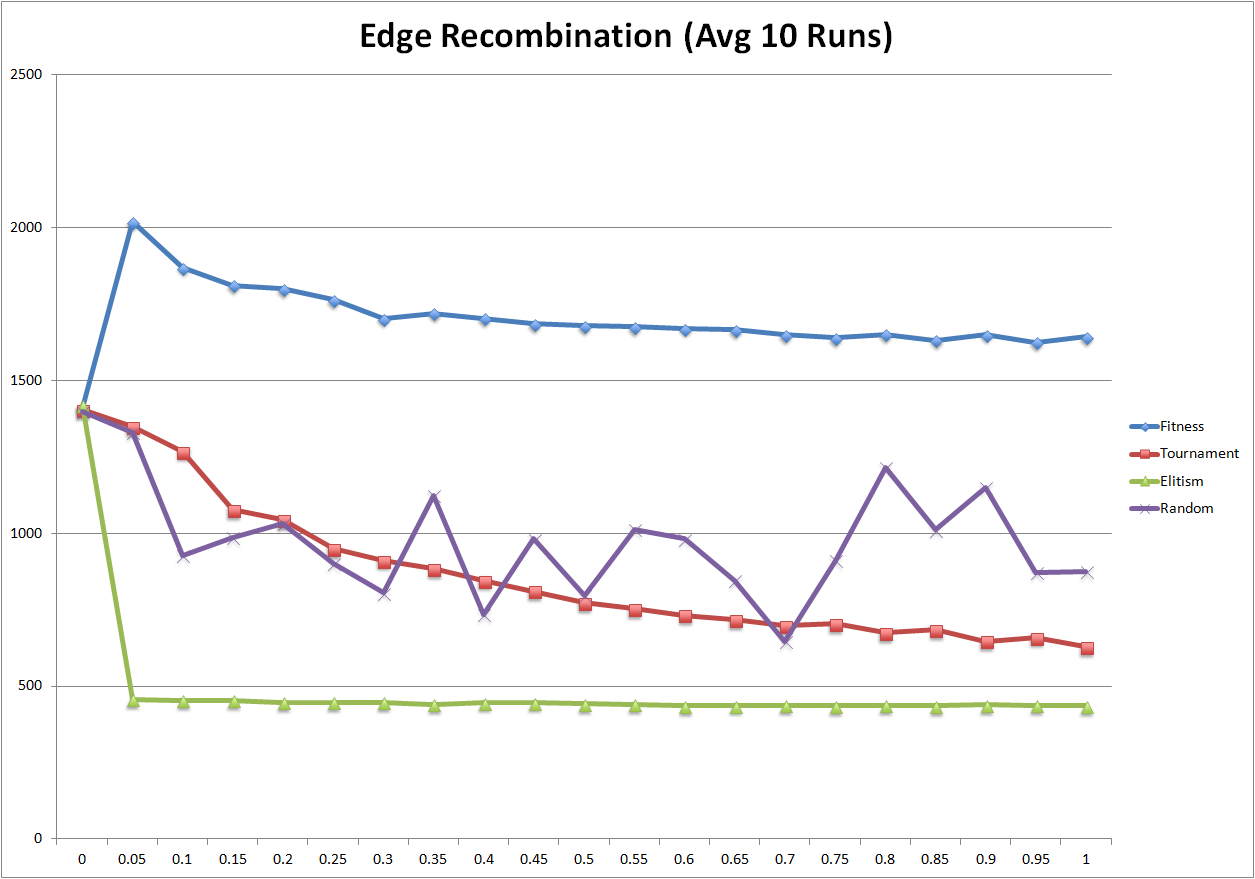
\includegraphics[width=12.5cm]{Edge.png}
\caption{Edge Recombination solution accuracy at percentage levels}
\end{figure}

\newpage
\section{Algorithms}
The first two algorithms are similar to those found in the recommended text for this course (GA and GP). The team made some minor modifications to better reflect the results from the TSP.\\

The three algorithms are:
\begin{enumerate}
\item Genetic Algorithm (GA)
\item Genetic Programming (GP)
\item Statistical Advantage\\
\end{enumerate}

*NOTE: For testing, each algorithm was run at least 10 times for each population/generation pair. The log files associated with these testing runs can be found in the main project files, split into appropriate files and folders. Due to the format of the log files, please ensure you fully expand ``column A'' when looking at the data to capture all related information. 

\subsection{A Modification to GA}
The Genetic Algorithm (GA) has the potential to perform mutation and cross-over operations sequentially, based on specific probabilities. The steps below explain the process for our use of the GA.\\

For each generation:
\begin{enumerate}
\item Select the best of the current population, duplicate it and set it aside.
\item Choose two individuals at random.
\item While the current population size is less than the maximum population size, do the following
\item Perform a cross-over, based on probability \textit{Pc} (creates two new children).
\item Perform a mutation (on the same set), based on probability \textit{Pm}.
\item Add the children back into the population and continue from step 3.
\item If the current population size is equal to the maximum population size, perform a selection method, chosen based on probability \textit{Ps}.
\item Start the next generation at step 1 until maximum number of generations reached.
\end{enumerate}
  
\newpage
\subsection{A Modification to GP}
Unlike the GA, the Genetic Programming (GP) approach has the potential to perform mutation OR cross-over methods seqentially, based on specific probabilities (but not both). The steps below explain the process for our use of the GP.\\

For each generation:
\begin{enumerate}
\item Select the best of the current population, duplicate it and set it aside.
\item Choose two individuals at random.
\item While the current population size is less than the maximum population size, do the following
\item Given a probability \textit{Pc} perform either a cross-over OR \textit{(1-Pc)} - the probability that a mutation would be chosen - for this entire generation. Either:
\begin{itemize}
	\item Perform a cross-over on the two individuals (creates two new children).
	\item Duplicate a single individual from the two randomly chosen and perform a mutation (creates a single new child).
\end{itemize}
\item Add the children back into the population and continue from step 3.
\item If the current population size is equal to the maximum population size, perform a selection method, based on probability \textit{Ps}.
\item Start the next generation at step 1 until maximum number of generations reached.\\
\end{enumerate}

Both these algorithms obtain good approximations, with the GA traditionally finding the solution faster. However since the GP has the possibility to retain a wide range solutions, it generally has marginally better results.

\newpage
\subsection{Statistical Advantage}
Using the statistics mentioned in the introduction, the team took the best aspects of algorithms 1 \& 2 and forumalted a new approach using very specific statistics.

For each generation:
\begin{enumerate}
\item Select the best of the current population, duplicate it and set it aside.
\item Clone the current population to form a ``mutants'' population
\item Clone the current population to form a ``cross-over'' population
\item For every individual in the ``mutants'' population:
\begin{itemize}
	\item Perform inversion 50\% of the time
	\item Perform insert or swap 45\% of the time
	\item Perform scramble the remaining 5\%
	\item Add the mutated children back into the population
\end{itemize}
\item Until the cross-over population is empty, choose two individuals at random and remove them from the cross-over population. Then do:
\begin{itemize}
	\item Edge Recombination 40\% of the time
	\item Order Crossover 30\% of the time
	\item PMX Crossover 20\% of the time
	\item Cycle Crossover the remaining 10\%
	\item Add the children back into the population
\end{itemize}
\item Perform a selection method:
\begin{itemize}
	\item Elitism and Tournment 95\% of the time
	\item Fitness-Proportional the remaining 5\% of the time
\end{itemize}
\item Start the next generation at step 1 until maximum number of generations reached.\\
\end{enumerate}

While this method is moderately slower then algorithm 1 and 2, with smaller population sizes (20 or less) this algorithm can generate solutions that are 15\% more accurate. With population sizes more than 20, solution accuracy ranges from 1 - 0.1\%, but what we observed was that this algorithm took considerably less generations to find an accurate solution. 

\newpage
\section{Issues}

\subsection{Infinite Looping on Small Populations}
With smaller populations there is the potential for an infinite loop in each of the algorithms. It is unknown where the issue occurs as it is very intermittent but the most likely cause is that the tours very quickly become equal. This is not through solution duplication but simply each of them individually finding the same solution through our TSP methods.\\

This has since been rectified but not extensively tested and thus deserves mentioning in this report. If duplicates are detected they are mutated to form new solutions. However the affect on run-time has also not been extensively studied.

\subsection{Fitness-Proportional}
During our test runs it was discovered that the Fitness-Proportional (FP) selection method was performing a maximisation rather than a minimisation. This  greatly affected our results and the choice of its use in our algorithms. This issue has since been rectified but there was not sufficient time to re-run the tests.

\subsection{Inver-Over Algorithm}
The Inver-Over operator discussed in the supplied paper produced some of the more accurate solutions. Our implementation gives good results but indications show results could be improved. Further analysis of its implementation would be required to rectify any issues found, but at this late stage its results are accurate enough for us to publish in this report.\\

As a side note, Inver-Over also appears to be the slowest algorithm from the three implemented and this factor should be considered when looking at the accuracy of solutions.

\subsection{Pr2392}
This data set is the largest of those supplied and took ~ 7 hours to run for a population size 50 at 10,000 generations. While we produced some data, only small portions are available and were only run once for each population/generation pair. More time spent in code review may produce faster methods and algorithms and would also allow us to perform additional tests.

\newpage
\section{Results}
A large portion of data has been left off this report for simplicity and succinctness. The log files containing this data can be found in the relevant folders of this project. The following tables reference population sizes of 50 and 100. Tables using population sizes of 10 and 20 can be found in the Appendix.

\subsection{Algorithm 3 - Statistical Advantage}
\begin{figure}[h]
\centering
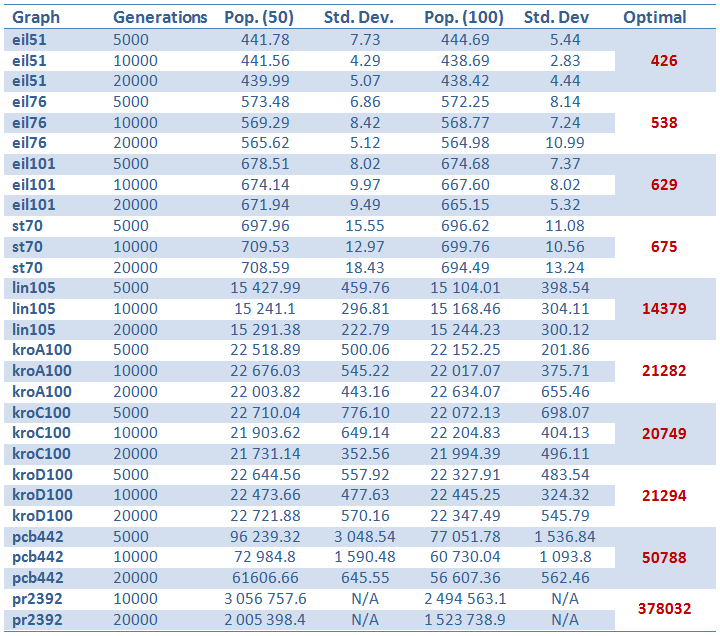
\includegraphics[width=\linewidth]{Alg3_Pop50_100.png}
\caption{Algorithm 3 average tour length for each population/generation pair, including standard deviation}
\end{figure}

\newpage
\subsection{Inver-Over}
\begin{figure}[h]
\centering
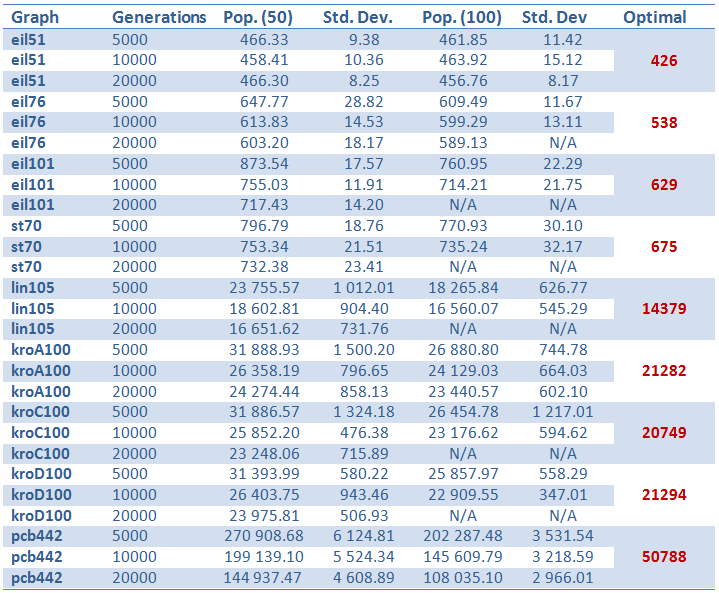
\includegraphics[width=\linewidth]{IV_Pop50_100.png}
\caption{Inver-Over algorithm average tour length for each population/generation pair, including standard deviation}
\end{figure}

\newpage
\section{Conclusion}
Given these results we found that while our algorithm takes slightly longer to complete than others, it does produce more accurate results and generally obtains them at a lower generation. Improvements to the code may render faster run times and more accurate results. Many of our methods changed after we ran the statistical analysis of the mutators and operators and this would change how our algorithms perform.\\

The Inver-Over algorithm produces its best results with larger populations and even larger generations. Issues in our implementation may have lead to the notion that our algorithms performed marginally better than the results produced with Inver-Over.\\

In addition, the algorithms above have the potential to produce tours that are similar or even the same. Further research must be done in order to combat this problem in a suitable run-time. Lastly, investigations into starting with potential (rather than random) solutions may also increase solution accuracy with less generations. Our results from running the pr2392 data set shows that an increase in generations would yield even better results.

\appendix
\newpage
\section{Algorithm 3 - Population sizes 10 and 20}
\begin{figure}[h]
\centering
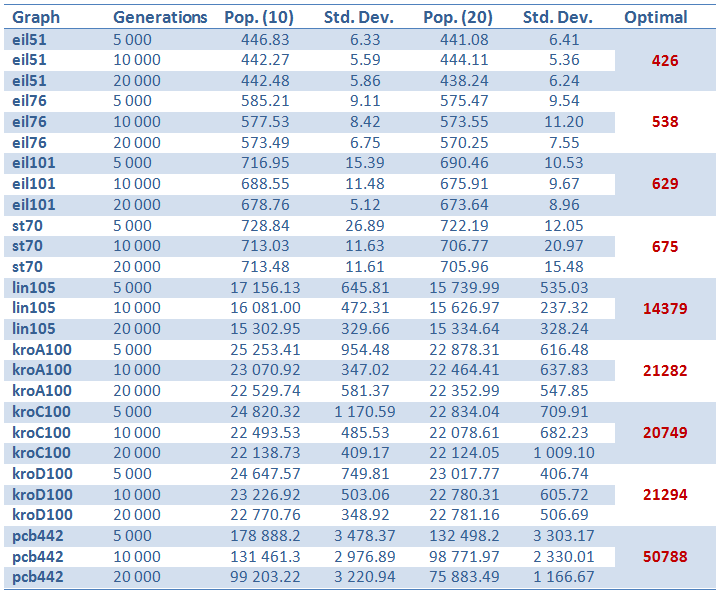
\includegraphics[width=\linewidth]{Alg3_Pop10_20.png}
\caption{Algorithm 3 average tour length for each population/generation pair, including standard deviation}
\end{figure}

\newpage
\section{Inver-Over Algorithm - Population sizes 10 and 20}
\begin{figure}[h]
\centering
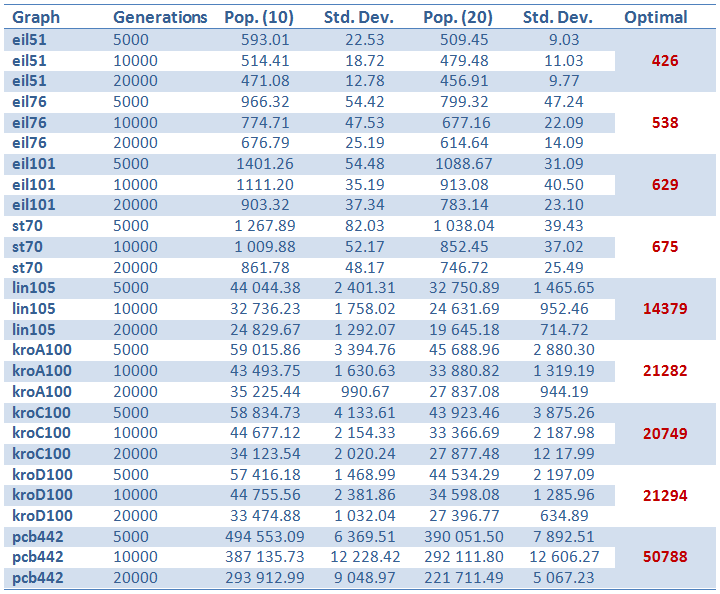
\includegraphics[width=\linewidth]{IV_Pop10_20.png}
\caption{Inver-Over algorithm average tour length for each population/generation pair, including standard deviation}
\end{figure}

\end{document}
